\section{Overview}
Since we're talking about learning without neurons, perhaps we should talk about what we mean about making computation. Murugan states there are two types of computation
\begin{enumerate}
	\item Symbolic: These are analytic expressions which a compute can crunch / a human can set 
	\item Behavior: Living organism / smart materials which respond and interact with their environment.
\end{enumerate}
The talk will focus on the latter. However computations are used to solve problems, so let's also define some ways of solving problems. Let's work through an example of heating and cooling a room with an AC. 
\begin{enumerate}
	\item Abstraction First:
	
	An example of this is PI control. So you set up a control flow.
	\begin{figure*}[h!]
		\centering
		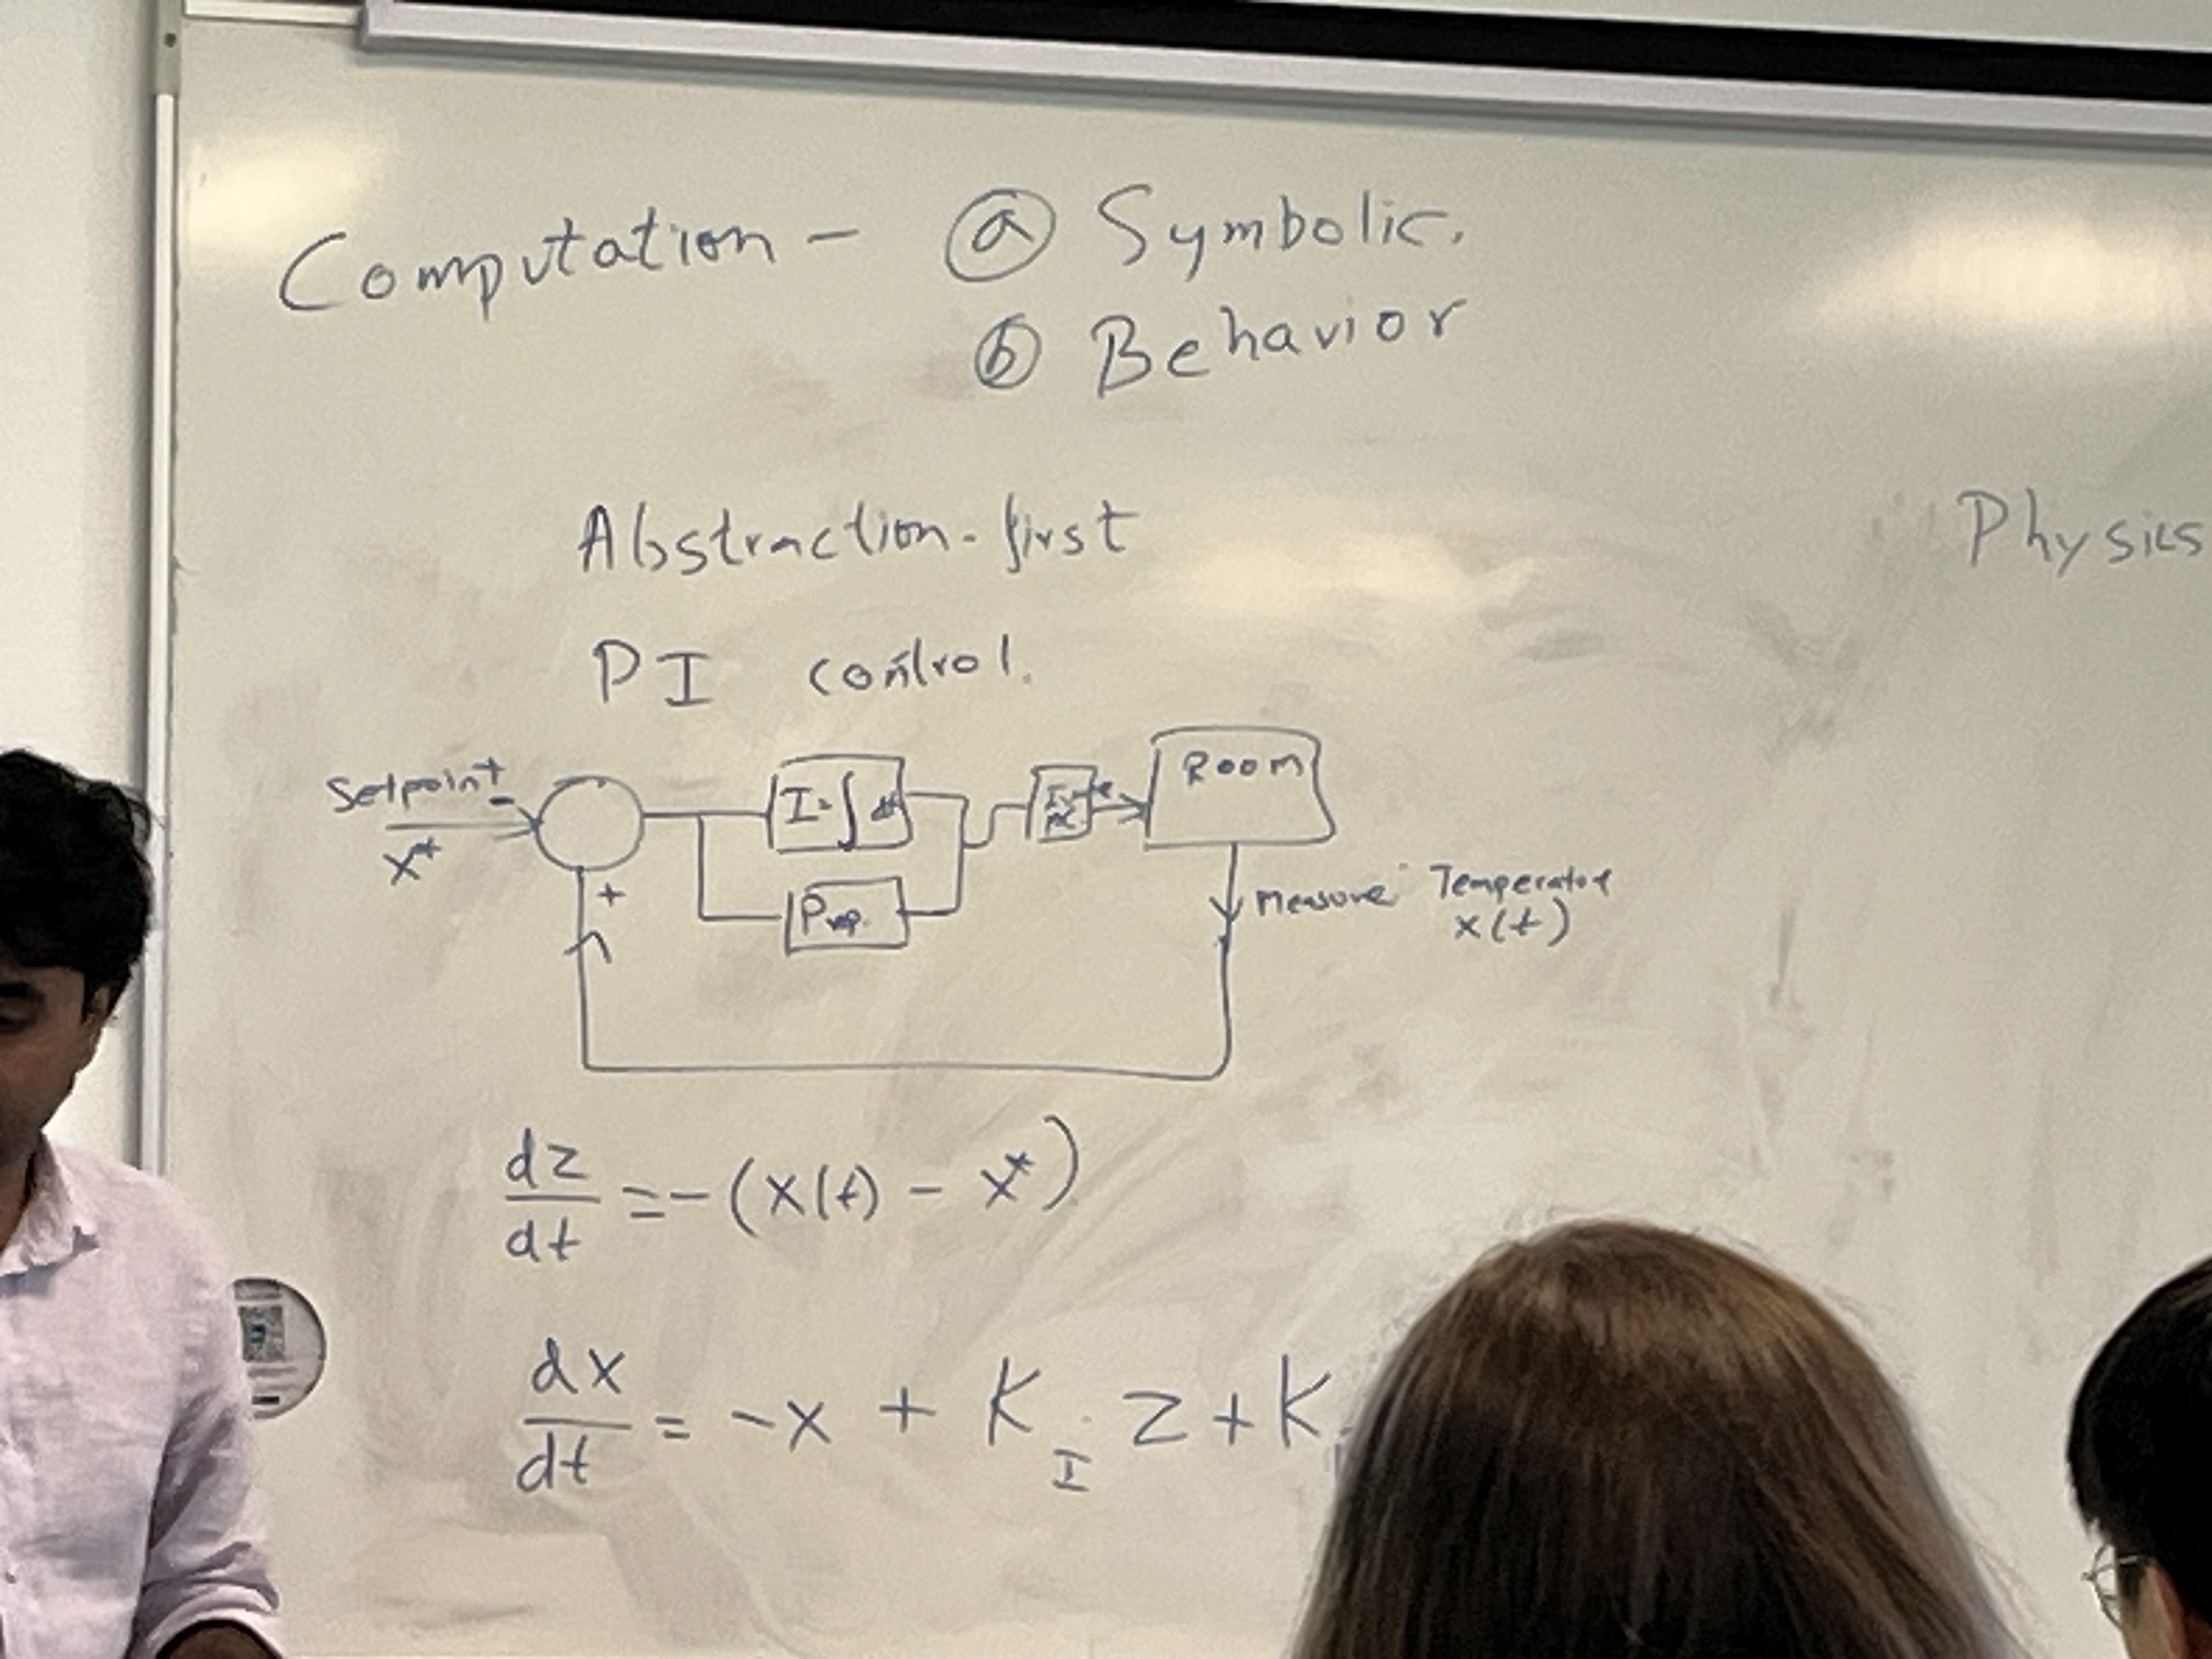
\includegraphics[scale=0.07]{figures/murugan/PI_Control.jpg}
		\caption{Diagram of control line}
	\end{figure*}\\
	This defines a differentiation equation which defines your control line $z$ due to observation of a process $x$
	\begin{itemize}
		\item Pros:
			\item General / modular
		\item Cons
			\item Cannot exploit specific physics
			\item The translation between theory vs implementation is non-trivial.
	\end{itemize}
	
	\item Physics First: 
	
	You can set up a thermodynamic state equation, and solve for the phase diagram.
	Pros and Cons
	\begin{itemize}
		\item Pros: 
			\item Fewer parts (measurement, computation), which means its more robust
			\item It's passive, meaning it self computes
		\item Cons
			\item Specific to the physics
	\end{itemize}
\end{enumerate}
This talk will focus on how to move toward the 2nd way of thinking. An example of this is the Liquid-Liquid phase transition of two liquids inside of a cell (see Zechnor 2020). You can think of this as oil and water separating.
\\
\\
There are two communities working on this
\begin{enumerate}
	\item Energy efficient computations (vs silicon). 
	\begin{itemize}
		\item Example. We currently run computations on a silicon chip, however this is not energy efficient, so much so governments are thinking about building more nuclear reactors to power the next generation of AI). So perhaps we can build biological circuits which run these computations natively on some bio-efficient chip.
		\item Example. Encode your optimization problem onto a Ising-like physical system, and anneal that system! Now you can read off optimized parameters.
		\item Example. You can use optimal computing to make better matrix multiplication.
	\end{itemize}
	\item Biological computations
	\begin{itemize}
		\item Backprop. That is each organism is reacting and adjusting it's behavior. Much more complex than just physics or chemical behavior.
		\item Evolution. No one organism does the computation, but rather it's the ensemble of them which can perform computations.
		\item Physics / Chemistry. It's just a reaction based on laws of physics / chemistry.
	\end{itemize}
\end{enumerate}
Now, how does this all relate to machine learning. Let's consider a high dimensional classifier-- you could think of the decision boundary as phase boundaries. You can also go one step further and use the transition between phases as the classifier (see \url{https://www.jbc.org/article/S0021-9258(20)36794-6/pdf} for more details)! So your features correspond to temperature, pressure, etc., and your classification is the phase. 
\begin{figure*}[h!]
	\centering
	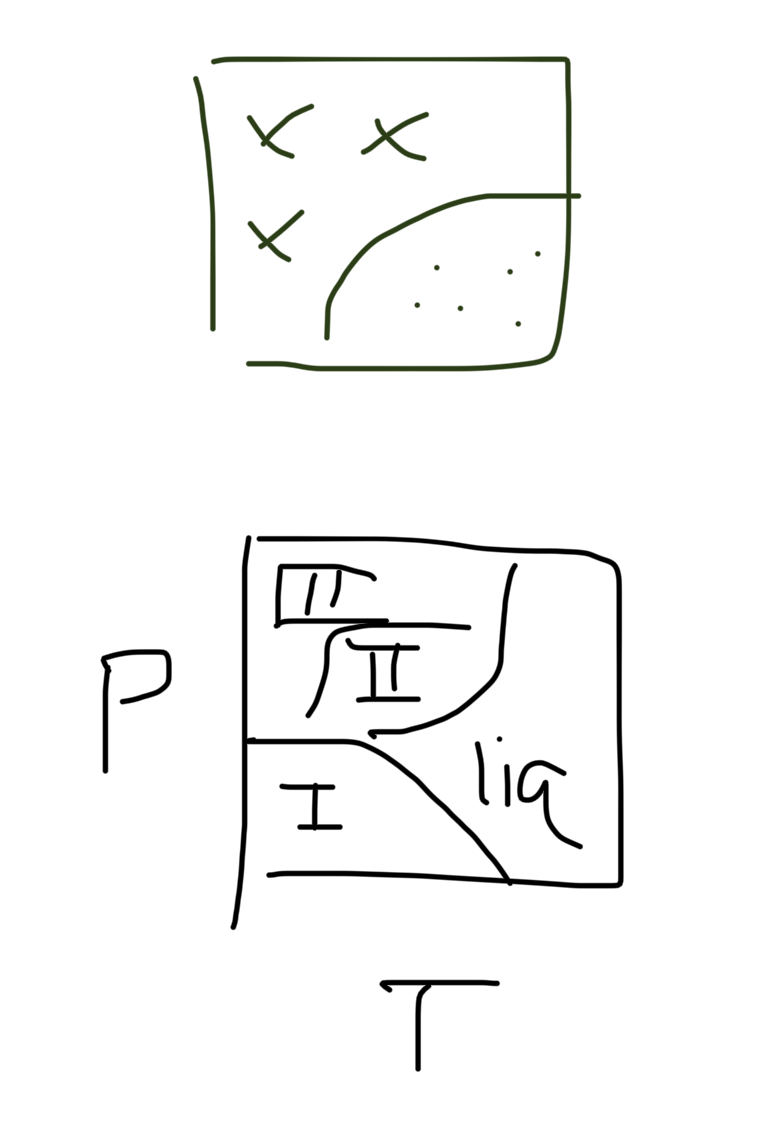
\includegraphics[scale=0.5]{figures/murugan/DecisionBoundary_PhaseDiagram.png}
	\caption{Decision boundary problems can be mapped into a physics system by inspecting their phase transition}
\end{figure*}
So the questions become what in the material / organism do I have to tune s.t. you can learn, and this also may find new interesting physical mechanisms for scientists to play with.

\subsection{Training Molecules}
\subsubsection{Hopefield Associative Memory}
Consider a set of neurons $\{x_i\}^N_{i=1}$ which take on binary values $x_i \in \{\pm 1\}$.  It takes on discrete dyanmics
\begin{align}
	x_i(t+1) = \text{sign}\left(\sum_j J_{ij} x_j(t) + h_i^{ext}(t) 
\right)
\end{align}
Your task is a supervised learning problem... The goal is to store a set of memories $m_i^\alpha \in \mathbb R^N$ (s.t. $\alpha = 1,..., M$). And you want to retrieve a memory $m$ from a just showing a partial part of $m$ (association). That is you want your neurons $\{x_i\}$ to fire in the same pattern as $m$ \\
\\
To train this model, we use a \textbf{Hebbian} learning rule
\begin{align}
	\frac{dJ_{ij}}{dt} = x_i (t) x_j(t)
\end{align}
We run this every time we should it a new memory. So for example, after being exposed to 3 memories $\{m^{(1)}, m^{(2)}, m^{(3)}\}$, our couplings look like $J_{ij} = m_i^{(1)} m_j^{(1)} + m_i^{(2)} m_j^{(2)} + m_i^{(3)} m_j^{(3)}$. Running this process will make the energy landscape become low where $x = m^{(i)}$-- so if you train on images, and then show noised versions of those images, then you'll be-able to denoise said images! Very cool! 

Note that hopfield networks have a memory capacity $M_c$, so this only works when the total memories $M < M_c$.

\subsubsection{Multifavious Assembly Mixtures}
Here we'll consider a physical system which is analogous to Hopfield's Assocative Memory model.

Consider $N$ molecular species in a solvent (this is different from the number of molecules, for example these can be $N$ proteins with different names), with binding interactions $J_{ij}$, and concentrations $C_i(x,t)$ at position $x$ at time $t$ (and associated chemical potentials $\mu_i$). The molecules are held at a physical temperature $T$, and have diffusion constant $D_i$.

\begin{align}
	\frac{dJ_{ij}}{dt} = - \int d^3x ~dt ~ C_i(x,t) C_j(x,t)
\end{align}
This rule says, these molecules will increase their bond ($J_{ij}$ will increase) if there are more of said molecules in the same place ($C_i(x,t) C_j(x,t)$ is the concentrations of molecules $i$ and $j$ at position $x$ at time $t$).

In practice, we need to use \textbf{linkers} (these are other molecules which mediate interactions between molecules). So they can be used to tune your $J_{ij}$'s. You can think of this has having a large interaction matirx $J$ (say 100 molecules), but you only observe a fraction of them yielding a tunable effective interaction matrix $\tilde J$ (say you actually only observe 10 molecules).

The associative memory is to reconstruct a set of protein binded together. So you can construct a memory as a sequence of proteins, cut it up, place it into the test tube, and see if it can reconstruct the previous protein.

\section{Expressitivity and Trainability}
Now that we've covered a one to one mapping between a machine learning method and a biological system which has a similar.
\subsection{Training of Molecular Networks}
We can train molecular networks using the sleep-wake algorithm. At a high-level, the algorithm is similar to the expectaiton-maximization algorithm. In this case, you have two distributions defined by a Spin-Glass like distribution, one is trainable $Q_{w}$ and the other is target distribution $P$, you update your couplings $w$ according to the difference of two point functions.
\begin{align}
	\frac{\partial D_{KL}(Q_{w} || P)}{\partial w_{ij}} = \underbrace{\langle s_i s_j \rangle_P}_{\text{sleep}} - \underbrace{\langle s_i s_j \rangle_Q}_{\text{wake}}
\end{align}


\subsection{Potts Model of Molecular Networks}
So, perhaps to make things more concrete, let's try to create a model of a molecular network. The molecules live in a test tube, so all interactions must occur at some real space $x \in \Lambda \subset \mathbb R^3$.  Consider the Potts Model. Configurations are which specifies of molecules $[N]=\{1,...,N\}$ are where, so the configurations are $\sigma: \Lambda \to [N]$. 
\begin{align}
	E = \sum_{x \in \Lambda} \sum_{x_n \in \partial x} J_{\sigma(x), \sigma(x_n)} + \sum_i \mu_i n_i(\sigma)
\end{align}
Where $J_{ij}$ is an interaction matrix between species (so $i = 1,..., N$ number of species), $\sum_{x_n \in \partial x}$ is a sum over the spatial neighbors of $x$, $\mu_i = - \log c_i$ is the chemical potential of species $i$ (which is the negative log of the concentration, and $n_i$ is the number of species at $\sigma$.

\subsection{Place Models}
Consider an Ising model of $N$ spins on a lattice. The place model now does all possible permutations of the spins with the same lattice structure.




















\newpage

